\documentclass{standalone}
\usepackage{tikz}
\usetikzlibrary{patterns, positioning}

\begin{document}
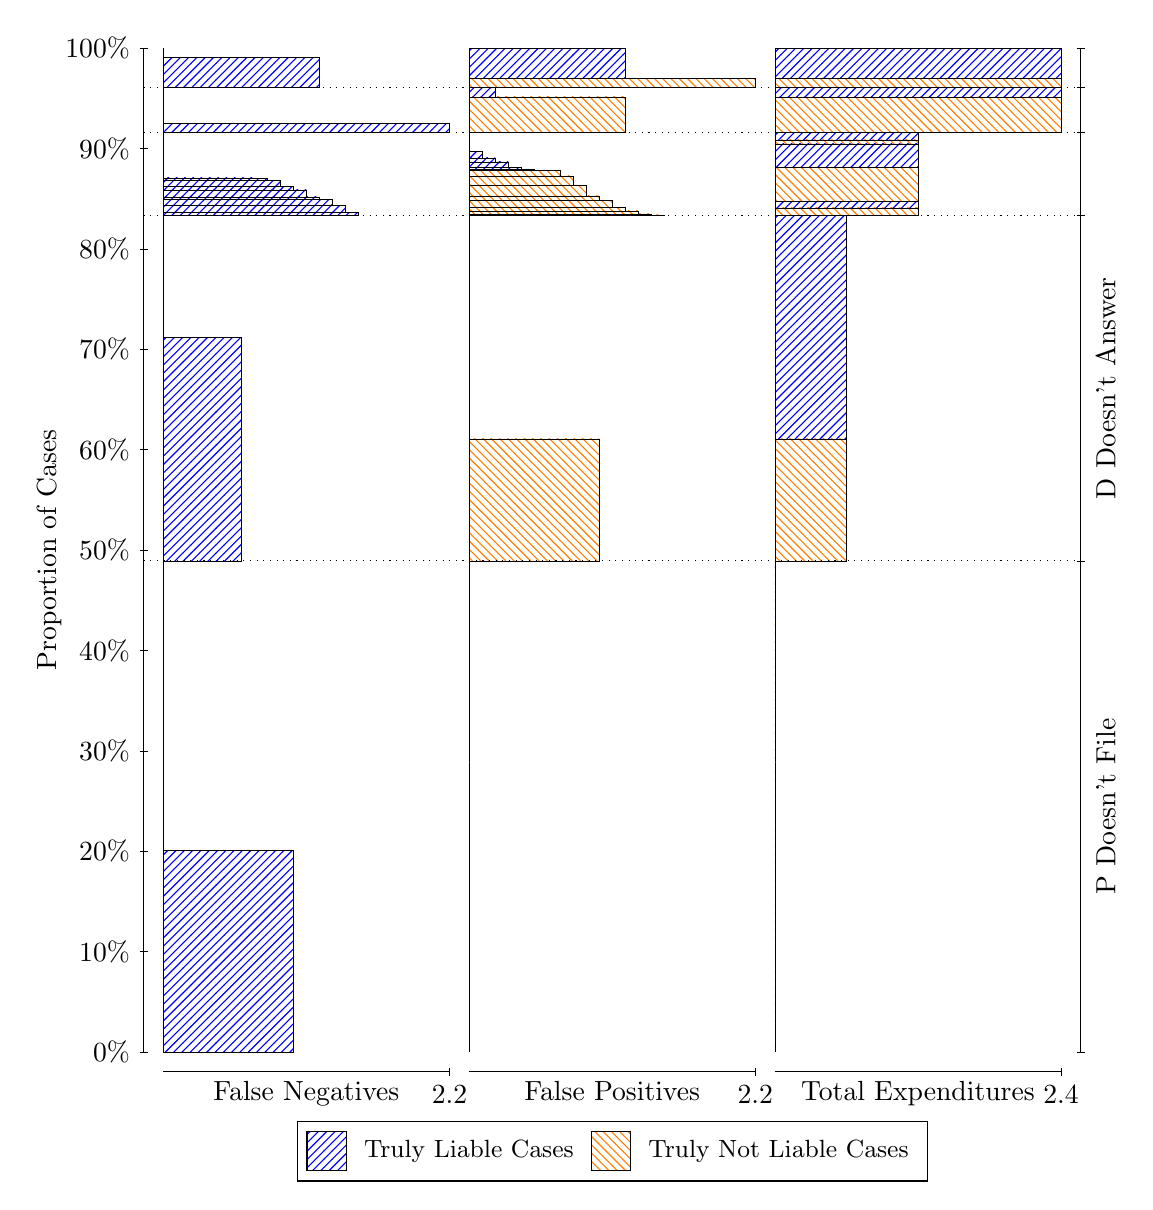
\begin{tikzpicture}
\draw[black, very thin] (1.5,1.75) -- (1.5,14.5);
\node[rotate=90, anchor=center] at (0.3, 8.125) {Proportion of Cases};
\draw[black, very thin] (1.45,1.75) -- (1.55,1.75);
\node[anchor=east] at (1.45, 1.75) {0\%};
\draw[black, very thin] (1.45,3.025) -- (1.55,3.025);
\node[anchor=east] at (1.45, 3.025) {10\%};
\draw[black, very thin] (1.45,4.3) -- (1.55,4.3);
\node[anchor=east] at (1.45, 4.3) {20\%};
\draw[black, very thin] (1.45,5.575) -- (1.55,5.575);
\node[anchor=east] at (1.45, 5.575) {30\%};
\draw[black, very thin] (1.45,6.85) -- (1.55,6.85);
\node[anchor=east] at (1.45, 6.85) {40\%};
\draw[black, very thin] (1.45,8.125) -- (1.55,8.125);
\node[anchor=east] at (1.45, 8.125) {50\%};
\draw[black, very thin] (1.45,9.4) -- (1.55,9.4);
\node[anchor=east] at (1.45, 9.4) {60\%};
\draw[black, very thin] (1.45,10.675) -- (1.55,10.675);
\node[anchor=east] at (1.45, 10.675) {70\%};
\draw[black, very thin] (1.45,11.95) -- (1.55,11.95);
\node[anchor=east] at (1.45, 11.95) {80\%};
\draw[black, very thin] (1.45,13.225) -- (1.55,13.225);
\node[anchor=east] at (1.45, 13.225) {90\%};
\draw[black, very thin] (1.45,14.5) -- (1.55,14.5);
\node[anchor=east] at (1.45, 14.5) {100\%};

\draw[black, very thin] (13.4,1.75) -- (13.4,14.5);
\draw[black, very thin] (13.35,1.75) -- (13.45,1.75);
\node[anchor=west] at (13.35, 1.75) {};
\draw[black, very thin] (13.35,7.9862) -- (13.45,7.9862);
\node[anchor=west] at (13.35, 7.9862) {};
\draw[black, very thin] (13.35,12.374) -- (13.45,12.374);
\node[anchor=west] at (13.35, 12.374) {};
\draw[black, very thin] (13.35,13.426) -- (13.45,13.426);
\node[anchor=west] at (13.35, 13.426) {};
\draw[black, very thin] (13.35,13.999) -- (13.45,13.999);
\node[anchor=west] at (13.35, 13.999) {};
\draw[black, very thin] (13.35,14.5) -- (13.45,14.5);
\node[anchor=west] at (13.35, 14.5) {};

\draw[black, very thin, pattern color=blue, pattern=north east lines] (1.75,1.75) rectangle (3.4015,4.3079);
\draw[black, very thin, pattern color=orange, pattern=north west lines] (1.75,4.3079) rectangle (1.75,7.9862);
\draw[black, very thin, pattern color=blue, pattern=north east lines] (1.75,7.9862) rectangle (2.7409,10.825);
\draw[black, very thin, pattern color=orange, pattern=north west lines] (1.75,10.825) rectangle (1.75,12.374);
\draw[black, very thin, pattern color=blue, pattern=north east lines] (1.75,12.374) rectangle (4.2273,12.412);
\draw[black, very thin, pattern color=blue, pattern=north east lines] (1.75,12.412) rectangle (4.0621,12.502);
\draw[black, very thin, pattern color=blue, pattern=north east lines] (1.75,12.502) rectangle (3.897,12.574);
\draw[black, very thin, pattern color=blue, pattern=north east lines] (1.75,12.574) rectangle (3.7318,12.609);
\draw[black, very thin, pattern color=blue, pattern=north east lines] (1.75,12.609) rectangle (3.5667,12.697);
\draw[black, very thin, pattern color=blue, pattern=north east lines] (1.75,12.697) rectangle (3.4015,12.747);
\draw[black, very thin, pattern color=blue, pattern=north east lines] (1.75,12.747) rectangle (3.2364,12.816);
\draw[black, very thin, pattern color=blue, pattern=north east lines] (1.75,12.816) rectangle (3.0712,12.842);
\draw[black, very thin, pattern color=blue, pattern=north east lines] (1.75,12.842) rectangle (2.9061,12.85);
\draw[black, very thin, pattern color=orange, pattern=north west lines] (1.75,12.85) rectangle (1.75,13.426);
\draw[black, very thin, pattern color=blue, pattern=north east lines] (1.75,13.426) rectangle (5.3833,13.544);
\draw[black, very thin, pattern color=orange, pattern=north west lines] (1.75,13.544) rectangle (1.75,13.999);
\draw[black, very thin, pattern color=blue, pattern=north east lines] (1.75,13.999) rectangle (3.7318,14.382);
\draw[black, very thin, pattern color=orange, pattern=north west lines] (1.75,14.382) rectangle (1.75,14.5);
\draw[black, very thin, pattern color=orange, pattern=north west lines] (5.6333,1.75) rectangle (5.6333,5.4283);
\draw[black, very thin, pattern color=blue, pattern=north east lines] (5.6333,5.4283) rectangle (5.6333,7.9862);
\draw[black, very thin, pattern color=orange, pattern=north west lines] (5.6333,7.9862) rectangle (7.2848,9.535);
\draw[black, very thin, pattern color=blue, pattern=north east lines] (5.6333,9.535) rectangle (5.6333,12.374);
\draw[black, very thin, pattern color=orange, pattern=north west lines] (5.6333,12.374) rectangle (8.1106,12.382);
\draw[black, very thin, pattern color=orange, pattern=north west lines] (5.6333,12.382) rectangle (7.9455,12.394);
\draw[black, very thin, pattern color=orange, pattern=north west lines] (5.6333,12.394) rectangle (7.7803,12.432);
\draw[black, very thin, pattern color=orange, pattern=north west lines] (5.6333,12.432) rectangle (7.6152,12.474);
\draw[black, very thin, pattern color=orange, pattern=north west lines] (5.6333,12.474) rectangle (7.45,12.568);
\draw[black, very thin, pattern color=orange, pattern=north west lines] (5.6333,12.568) rectangle (7.2848,12.622);
\draw[black, very thin, pattern color=orange, pattern=north west lines] (5.6333,12.622) rectangle (7.1197,12.76);
\draw[black, very thin, pattern color=orange, pattern=north west lines] (5.6333,12.76) rectangle (6.9545,12.877);
\draw[black, very thin, pattern color=orange, pattern=north west lines] (5.6333,12.877) rectangle (6.7894,12.95);
\draw[black, very thin, pattern color=blue, pattern=north east lines] (5.6333,12.95) rectangle (6.4591,12.958);
\draw[black, very thin, pattern color=blue, pattern=north east lines] (5.6333,12.958) rectangle (6.2939,12.985);
\draw[black, very thin, pattern color=blue, pattern=north east lines] (5.6333,12.985) rectangle (6.1288,13.053);
\draw[black, very thin, pattern color=blue, pattern=north east lines] (5.6333,13.053) rectangle (5.9636,13.104);
\draw[black, very thin, pattern color=blue, pattern=north east lines] (5.6333,13.104) rectangle (5.7985,13.191);
\draw[black, very thin, pattern color=blue, pattern=north east lines] (5.6333,13.191) rectangle (5.6333,13.426);
\draw[black, very thin, pattern color=orange, pattern=north west lines] (5.6333,13.426) rectangle (7.6152,13.88);
\draw[black, very thin, pattern color=blue, pattern=north east lines] (5.6333,13.88) rectangle (5.9636,13.999);
\draw[black, very thin, pattern color=orange, pattern=north west lines] (5.6333,13.999) rectangle (9.2667,14.116);
\draw[black, very thin, pattern color=blue, pattern=north east lines] (5.6333,14.116) rectangle (7.6152,14.5);
\draw[black, very thin, pattern color=orange, pattern=north west lines] (9.5167,1.75) rectangle (9.5167,5.4283);
\draw[black, very thin, pattern color=blue, pattern=north east lines] (9.5167,5.4283) rectangle (9.5167,7.9862);
\draw[black, very thin, pattern color=orange, pattern=north west lines] (9.5167,7.9862) rectangle (10.425,9.535);
\draw[black, very thin, pattern color=blue, pattern=north east lines] (9.5167,9.535) rectangle (10.425,12.374);
\draw[black, very thin, pattern color=orange, pattern=north west lines] (9.5167,12.374) rectangle (11.333,12.469);
\draw[black, very thin, pattern color=blue, pattern=north east lines] (9.5167,12.469) rectangle (11.333,12.557);
\draw[black, very thin, pattern color=orange, pattern=north west lines] (9.5167,12.557) rectangle (11.333,12.988);
\draw[black, very thin, pattern color=blue, pattern=north east lines] (9.5167,12.988) rectangle (11.333,13.282);
\draw[black, very thin, pattern color=orange, pattern=north west lines] (9.5167,13.282) rectangle (11.333,13.332);
\draw[black, very thin, pattern color=blue, pattern=north east lines] (9.5167,13.332) rectangle (11.333,13.426);
\draw[black, very thin, pattern color=orange, pattern=north west lines] (9.5167,13.426) rectangle (13.15,13.88);
\draw[black, very thin, pattern color=blue, pattern=north east lines] (9.5167,13.88) rectangle (13.15,13.999);
\draw[black, very thin, pattern color=orange, pattern=north west lines] (9.5167,13.999) rectangle (13.15,14.116);
\draw[black, very thin, pattern color=blue, pattern=north east lines] (9.5167,14.116) rectangle (13.15,14.5);
\draw[black, dotted] (1.5,7.9862) -- (13.4,7.9862);
\draw[black, dotted] (1.5,12.374) -- (13.4,12.374);
\draw[black, dotted] (1.5,13.426) -- (13.4,13.426);
\draw[black, dotted] (1.5,13.999) -- (13.4,13.999);
\draw[black, very thin] (1.75,1.5) -- (5.3833,1.5);
\node[anchor=north] at (3.5667, 1.5) {False Negatives};
\draw[black, very thin] (5.3833,1.45) -- (5.3833,1.55);
\node[anchor=north] at (5.3833, 1.45) {2.2};

\draw[black, very thin] (5.6333,1.5) -- (9.2667,1.5);
\node[anchor=north] at (7.45, 1.5) {False Positives};
\draw[black, very thin] (9.2667,1.45) -- (9.2667,1.55);
\node[anchor=north] at (9.2667, 1.45) {2.2};

\draw[black, very thin] (9.5167,1.5) -- (13.15,1.5);
\node[anchor=north] at (11.333, 1.5) {Total Expenditures};
\draw[black, very thin] (13.15,1.45) -- (13.15,1.55);
\node[anchor=north] at (13.15, 1.45) {2.4};

\node[black, centered, rotate=90] at (13.72, 4.8681) {P Doesn't File};
\node[black, centered, rotate=90] at (13.72, 10.18) {D Doesn't Answer};




\draw (7.449999999999999,1.5) node[draw=none] (baseCoordinate) {};
\begin{scope}[align=center]
        \matrix[scale=0.5, draw=black, below=0.5cm of baseCoordinate, nodes={draw}, column sep=0.1cm]{
            \node[rectangle, draw, minimum width=0.5cm, minimum height=0.5cm, pattern=north east lines, pattern color=blue] {}; &
            \node[draw=none, font=\small] (B) {Truly Liable Cases}; &
            \node[rectangle, draw, minimum width=0.5cm, minimum height=0.5cm, pattern=north west lines, pattern color=orange] {}; &
            \node[draw=none, font=\small] (B) {Truly Not Liable Cases}; \\
            };
\end{scope}

\end{tikzpicture}
\end{document}